\documentclass[10pt,conference]{IEEEtran}
\usepackage{cite}
\usepackage{amsmath}
\usepackage[T1]{fontenc}
\usepackage{graphicx}
\usepackage{url}
\usepackage{hyperref}
\usepackage{booktabs}
\usepackage{tabularx}
\usepackage{array}
\renewcommand{\topfraction}{0.95}
\renewcommand{\dbltopfraction}{0.95}
\renewcommand{\textfraction}{0.05}
\renewcommand{\floatpagefraction}{0.85}
\setcounter{topnumber}{4}
\setcounter{dbltopnumber}{3}
\setcounter{totalnumber}{6}
\begin{document}
\title{A Common Standard for Comparing Reviews of Artificial Intelligence Benchmarks}
\author{Anonymous authors}
\maketitle
\begin{abstract}
\textbf{Background:} At least seven frameworks have been proposed for reviewing AI benchmarks, but differing scopes, incompatible scales, and conflicting rules make their results difficult to compare.
\textbf{Objective:} We introduce MESA, a comparative standard for benchmark reviews, use it to evaluate six frameworks across four benchmarks and create the MESA rubric derived from their shared criteria.
\textbf{Method:} All 280 items from the seven frameworks were mapped to 30 shared criteria. Coding agents applied six frameworks to fixed snapshots of four benchmarks; answers were standardized into three verdicts (\emph{satisfied}, \emph{unsatisfied}, \emph{open}) with qualifiers isolating penalties for unstated information. Agents then applied the MESA rubric twice per benchmark, and an assistant model checked all 296 ratings against cited sources, with author verification.
\textbf{Results:} No criterion is shared by all seven frameworks, and five penalize unstated information by design. Standardized verdicts match on 53\% of shared criteria. Across 143 disagreements, 92 stem from item granularity or rules for undocumented items rather than conflicting readings of evidence. In agent answers, penalties for unstated information outnumber documented defects by >10:1, although limited code inspection likely under counts defects. The MESA rubric achieves 80\% repeatability across runs and records missing information as open questions; source verification confirmed 190 of 232 ratings, found 21 overstated, and found 18 of 64 description values overstated.
\textbf{Conclusion:} MESA provides a shared vocabulary that decouples reported defects from unstated practices, as well as a standardized rubric. Evaluating the rubric produced verifiable, source-grounded ratings for benchmark selection and audit.
\end{abstract}
\begin{IEEEkeywords}
benchmark review, review teams, measurement, evaluation frameworks, coding agents, evidence, software evaluation
\end{IEEEkeywords}

\section{Introduction}
Teams selecting or auditing an artificial intelligence benchmark must decide whether its tasks, grading procedures and documentation support the claims attached to its scores. Since 2023 at least seven frameworks have been proposed for reviewing benchmarks \cite{cohn_hernandez_orallo_oecd_2023,reuel_betterbench,liu_ecbd_2024,cao_how2bench_2025,zhu_agentic_benchmark_checklist_2025,san_joaquin_scorecard_2026,corona_benchmark_caliper_2026}. Applying them to the same benchmark exposes an obstacle: they share no common vocabulary, scale, or rule for unstated information.

Consider training data contamination. BetterBench asks two questions and scores 0 when sources say nothing \cite{reuel_betterbench}; How2Bench groups what the paper omits with what was not done \cite{cao_how2bench_2025}; the Scorecard marks unmentioned overlap unsatisfied \cite{san_joaquin_scorecard_2026}; the Agentic Benchmark Checklist (ABC) scores whether a private test set exists \cite{zhu_agentic_benchmark_checklist_2025}; and ECBD, Caliper, and the OECD framework do not ask at all \cite{liu_ecbd_2024,corona_benchmark_caliper_2026,cohn_hernandez_orallo_oecd_2023}. When a benchmark paper is silent on contamination, four frameworks record a failure and three say nothing. Readers cannot distinguish substantive agreement from divergent scoring conventions. The same problem arises within review teams: when two reviewers apply different frameworks to the same benchmark, they cannot pool their verdicts or discuss them on common terms.

Evidence-based medicine routinely tests study appraisal tools empirically. When Hartling et al.\ evaluated the Cochrane risk-of-bias tool and the Newcastle-Ottawa scale with independent reviewers, low inter-rater agreement traced back to ambiguous tool guidance rather than the underlying trials \cite{hartling_rand_2012}. We take a similar approach: benchmark review frameworks must be evaluated by applying them to identical benchmarks and tracing their disagreements to their wording, granularity, and scoring rules.

We introduce MESA (Meta-Evaluation Standard for AI) as a translation layer and review standard across the seven frameworks. MESA provides: (1) 30 shared review criteria mapping all 280 framework items; (2) three standardized verdicts (\emph{satisfied}, \emph{unsatisfied}, \emph{open}) with qualifiers isolating partial support (\emph{partial}) and negative scores from unstated items (\emph{undocumented}); (3) structured evidence records capturing verbatim quotes, locators, and checks performed; and (4) an instrument description using eight OECD facets \cite{cohn_hernandez_orallo_oecd_2023} to govern applicability. Together these give reviewers and teams a shared record of what each framework asked, what evidence was found, and why a verdict was reached.

We evaluate MESA across four benchmarks spanning diverse tasks: HumanEval (code synthesis) \cite{human_eval_repository}, TruthfulQA (hallucination and truthfulness) \cite{truthfulqa_repository}, Humanity's Last Exam (HLE, frontier knowledge) \cite{phan_etal_hle_2025}, and $\tau$-bench (tool-agent interaction) \cite{tau_bench_repository}. In Study~1, coding agents apply six frameworks to fixed snapshots, standardizing agent outputs and published reviews onto the 30 criteria. Using one agent model for every framework is a deliberate control: it holds the reviewer fixed, so that differences can be traced to the frameworks rather than to reviewers. In Study~2, agents apply the derived MESA rubric twice per benchmark (Part~A: 8 description facets; Part~B: 29 evaluation questions with 6 levels: \emph{Claimed}, \emph{Documented}, \emph{Verified}, \emph{Contradicted}, \emph{Undocumented}, \emph{Not applicable}). We investigate four research questions: \textbf{RQ1} (coverage across shared criteria); \textbf{RQ2} (cross-framework agreement on identical benchmarks, and agreement with the framework teams' own published reviews); \textbf{RQ3} (treatment of unstated information); and \textbf{RQ4} (source verification and repeatability of the MESA rubric).

Our contributions are the MESA standard, the mapping of all 280 items, the comparative analysis of coverage and unstated-information rules, the derived MESA rubric, and findings from 28 agent sessions with 232 source-verified ratings and 64 description values.

\section{Background and Related Work}
\subsection{Test review and score validity}
In psychological and educational measurement, validity is the degree to which evidence and theory support the interpretation and use of scores for a stated purpose \cite{kane_validation,aera_apa_ncme_standards_2014}. The 2025 version of the European Federation of Psychologists' Associations (EFPA) Test Review Model operationalizes this by separating neutral instrument description (purpose, administration, scoring mode and reference group) from anchored ratings of construct representation, reliability and validity support that keep missing documentation distinct from negative evidence \cite{efpa_test_review_model_2025}.

Cohn and Hern\'andez-Orallo adapted this taxonomic approach to AI evaluation instruments across 18 categorical facets under validity, consistency and fairness \cite{cohn_categorising_2022,cohn_hernandez_orallo_oecd_2023}. When four raters classified 20 instruments in the 2023 OECD study, they agreed consistently on observable design facets such as \emph{Judgeability} (manual, automated or mixed scoring) and \emph{Purpose} (research or conformity), but disagreed on a third to half of instruments on evaluative facets such as \emph{Coverage} and \emph{Specificity} \cite{cohn_hernandez_orallo_oecd_2023}.

\subsection{Frameworks for reviewing benchmarks}
We examine seven frameworks evaluating benchmarks as measurement instruments (Table~\ref{tab:frameworks}): \textbf{BetterBench (BB)} \cite{reuel_betterbench} scores 47 template items (46 in paper) across four lifecycle stages; the \textbf{ECBD worksheet} \cite{liu_ecbd_2024} asks 20 open-ended questions across seven modules without scores; the \textbf{Scorecard of AI Benchmark Quality (SC)} \cite{san_joaquin_scorecard_2026} evaluates 22 principles and 46 bullets across five validity dimensions; \textbf{How2Bench (H2B)} \cite{cao_how2bench_2025} provides a 55-item checklist across five phases for code benchmarks; the \textbf{Agentic Benchmark Checklist (ABC)} \cite{zhu_agentic_benchmark_checklist_2025} scores 44 released items (42 in paper) across task, outcome, and reporting validity; \textbf{Benchmark Caliper (CAL)} \cite{corona_benchmark_caliper_2026} evaluates regional transfer across 28 items and six dimensions; and the \textbf{OECD facets} \cite{cohn_hernandez_orallo_oecd_2023} classify instruments across 18 facets.

\begin{table*}[t]
\caption{The seven review frameworks and the MESA rubric.}
\label{tab:frameworks}
\centering
\footnotesize
\begin{tabularx}{\textwidth}{@{}l>{\raggedright\arraybackslash}p{2.6cm}rr>{\raggedright\arraybackslash}p{3.1cm}>{\raggedright\arraybackslash}XX@{}}
\toprule
\textbf{Code} & \textbf{Framework} & \textbf{Items in paper} & \textbf{Items in template} & \textbf{Scope} & \textbf{Rule for undocumented items} & \textbf{Resulting verdict} \\
\midrule
BB & BetterBench \cite{reuel_betterbench} & 46 & 47 & General AI benchmarks (4 lifecycle stages) & Unacknowledged item scored 0; mentioned without evidence scored 5 & Unsatisfied, \emph{undocumented} \\
ECBD & ECBD worksheet \cite{liu_ecbd_2024} & 20 & 20 & NLP benchmarks (7 modules) & Absence of justification or support recorded in text without score & Open \\
SC & Scorecard \cite{san_joaquin_scorecard_2026} & 68 & 68 & General AI benchmarks (5 validity dimensions) & Vague or absent documentation marks the item unsatisfied & Unsatisfied, \emph{undocumented} \\
H2B & How2Bench \cite{cao_how2bench_2025} & 55 & 55 & Code benchmarks (5 phases) & A step without explicit paper text is labeled not mentioned and grouped with not done & Unsatisfied, \emph{undocumented} \\
ABC & Agentic Benchmark Checklist \cite{zhu_agentic_benchmark_checklist_2025} & 42 & 44 & Agentic benchmarks (task, outcome, reporting) & An undocumented item is scored 0 & Unsatisfied, \emph{undocumented} \\
CAL & Benchmark Caliper \cite{corona_benchmark_caliper_2026} & 28 & 28 & Cultural/regional transfer (6 dimensions) & The item returns Unknown; the dimension rubric lowers the score to 1 or 2 when transfer is not discussed & Item open; dimension unsatisfied, \emph{undocumented} \\
OECD & OECD facets \cite{cohn_hernandez_orallo_oecd_2023} & 18 & 18 & All AI evaluation instruments (3 areas) & Reliability allows N/A when unclear; other facets require a listed value & Reliability open; five evaluative facets satisfied or unsatisfied; 13 descriptive facets not standardized \\
\midrule
--- & MESA rubric & --- & 37 & General AI benchmarks (8 facets + 29 questions) & An undocumented item is recorded as \emph{Undocumented}, with the missing information noted & Open \\
\bottomrule
\end{tabularx}
\par\vspace{2pt}\raggedright\footnotesize Items in paper: the item count the framework's paper states; items in template: the items its released template or checklist contains, which we transcribed. Answer scales and their standardization are given in Section~\ref{sec:verdicts}.
\end{table*}

These frameworks serve diverse purposes: ECBD is a design worksheet, OECD classifies instruments, Caliper assesses transfer, and BetterBench, How2Bench, Scorecard, and ABC audit practice and documentation. MESA groups their questions by review concern. Questions in the same group can address different requirements: an estimator, a confidence interval, and a sampling description all concern statistical support without substituting for one another. Frameworks are compared only on criteria both cover, retaining original questions and answers alongside translated verdicts. Related templates such as Evaluation Cards structure evaluator reporting \cite{ghosh_evaluation_cards_2026}, while the Benchmark Health Index computes leaderboard statistics without inspecting documentation \cite{zhu_benchmark_health_index_2026}. No benchmark in our corpus possesses published reviews from multiple framework teams.

\subsection{Automated task auditing and comparative appraisal}
Automated auditors inspect individual benchmark tasks and execution traces for broken tests, label errors, or environment leaks \cite{tu_benchguard_2026,wang_auto_benchmark_audit_2026,suh_agentsuite_2026,mohl_transcript_flaws_2026,skarlinski_futurehouse_hle_2025}. In contrast, we examine frameworks reviewing benchmarks as measurement instruments, using known implementation properties to test whether reviewers inspect code alongside papers. Following medical appraisal studies that test review instruments by applying them across studies \cite{hartling_rand_2012,woelfle_appraisal_llm_2024,vanderkuil_checklist_disagreement_2026,dashti_quadas2_2026}, we adapt shared-criterion mapping, disagreement-cause coding, and source verification for every rating.

\section{The Standard and the MESA Rubric}
Eight terms have fixed meanings throughout: a \emph{framework} is a published set of benchmark review questions; a \emph{criterion} is one of the 30 shared rows; an \emph{answer} is a reviewer's response to one framework item and a \emph{rating} is its response to one rubric question; a \emph{verdict} is the standardized form of one or more answers on a criterion (\emph{satisfied}, \emph{unsatisfied} or \emph{open}); a \emph{session} is one coding agent applying one framework or the rubric to one snapshot; a \emph{published review} is a framework team's own published review of a benchmark; and the \emph{assistant model} is the model (Claude Fable 5.1, from the same model family as the Claude Sonnet 5.5 session reviewer) disclosed at the end.

\subsection{Shared criteria}
All 280 items across the seven frameworks were transcribed with their verbatim text (or marked paraphrase where sources give only prose), scale, rule for undocumented items and source location. Rather than imposing a fixed taxonomy, we expanded an initial list of 22 measurement criteria \cite{aera_apa_ncme_standards_2014,kane_validation,efpa_test_review_model_2025} bottom up to the 30 criteria listed in Table~\ref{tab:coverage}, from the construct and intended use (C01--C03) through validity, repeatability and reporting criteria to descriptive instrument classification (C30).

To keep the mapping transparent in a single-author study, the assistant model first generated a draft mapping for all 280 items, the author then mapped all 280 items independently without viewing the draft, and finally the author compared the two mappings and recorded a written reconciliation for every difference. All three columns are published.

\subsection{Three verdicts, qualifiers and answerability}
\label{sec:verdicts}
\begin{table}[t]
\caption{Standardization rules for verdicts and qualifiers.}
\label{tab:standardization}
\centering\scriptsize
\setlength{\tabcolsep}{3pt}
\begin{tabular}{@{}lllll@{}}
\toprule
\textbf{Framework} & \textbf{Answer} & \textbf{Evidence} & \textbf{Verdict} & \textbf{Qualifier} \\
\midrule
BetterBench & 15 & -- & Satisfied &  \\
 & 10 & -- & Satisfied & partial \\
 & 5 & -- & Unsatisfied & undocumented \\
 & 0 & undocumented & Unsatisfied & undocumented \\
 & 0 & contradicted & Unsatisfied &  \\
 & n/a & -- & Open & n/a \\
\midrule
ECBD & free text & documented & Satisfied &  \\
 & free text & undocumented & Open &  \\
 & free text & contradicted & Unsatisfied &  \\
\midrule
Scorecard & satisfied & -- & Satisfied &  \\
 & unsatisfied & undocumented & Unsatisfied & undocumented \\
 & unsatisfied & contradicted & Unsatisfied &  \\
 & n/a & -- & Open & n/a \\
\midrule
How2Bench & present & -- & Satisfied &  \\
 & not mentioned & -- & Unsatisfied & undocumented \\
\midrule
ABC & 1 & -- & Satisfied &  \\
 & 0 & undocumented & Unsatisfied & undocumented \\
 & 0 & contradicted & Unsatisfied &  \\
 & 0 or 1 & no tools & Open & n/a \\
\midrule
Caliper & 4 or 5 & -- & Satisfied &  \\
 & 3 & -- & Satisfied & partial \\
 & 1 or 2 & undocumented & Unsatisfied & undocumented \\
 & 1 or 2 & contradicted & Unsatisfied &  \\
 & Unknown & -- & Open &  \\
\midrule
OECD (5 facets) & preferred & -- & Satisfied &  \\
 & other & -- & Unsatisfied &  \\
 & N/A & -- & Open &  \\
\midrule
OECD (13 facets) & any & -- & Not standardized & descr. \\
\midrule
Rubric & Verified & -- & Satisfied &  \\
 & Documented & -- & Satisfied & partial \\
 & Claimed & -- & Satisfied & partial \\
 & Contradicted & -- & Unsatisfied &  \\
 & Undocumented & -- & Open &  \\
 & Not applicable & -- & Open & n/a \\
\bottomrule
\end{tabular}
\par\vspace{2pt}\raggedright\footnotesize Evidence: what the reviewer found in the sources; -- means the rule does not consult it. Verdict: the shared three-way result. Qualifier: why the verdict was reached; \emph{undocumented} ($-r$) means the unsatisfied verdict follows only from the framework's rule for an undocumented item; \emph{partial}: intermediate support; n/a: not applicable; descr.: descriptive facet, not standardized.
\end{table}

Each item answer captures four fields: the reviewer's \emph{answer} (the framework's native score); observed \emph{evidence} (\emph{documented}, \emph{undocumented}, \emph{contradicted}, or \emph{not applicable}); the standardized three-way \emph{verdict} (\emph{satisfied}, \emph{unsatisfied}, \emph{open}); and a \emph{qualifier} preserving the rationale (\emph{partial} for intermediate support; \emph{undocumented} for negative scores triggered solely by absent reporting). Pre-declared rules (Table~\ref{tab:standardization}) standardize every answer. When multiple items map to a criterion, verdicts aggregate deterministically: (1) if any mapped item is \emph{unsatisfied}, the criterion is \emph{unsatisfied} (qualified as \emph{undocumented} iff all unsatisfied items carry it); (2) else if all mapped items are \emph{satisfied} without \emph{partial}, it is \emph{satisfied}; (3) else if at least one mapped item is \emph{satisfied}, it is \emph{satisfied} (\emph{partial}); (4) otherwise \emph{open}.

An audit of all 280 items found 238 answerable from static documents and code, 25 Caliper items answerable once a target region is declared, 11 partly answerable (e.g., build badges), and 6 unanswerable (BB-45/46, H2B-45, CAL-IC-4, CAL-OO-4, CAL-OC-4, concerning live maintenance or porting teams). Unanswerable items are excluded identically from criterion verdicts in agent and published reviews; the item-level agent answer counts in Sections~\ref{sec:rq2} and~\ref{sec:rq3} still include the three unanswerable items of the applied frameworks (BB-45/46, H2B-45).

\subsection{Answer record, Part A description and Part B rubric}
\label{sec:evidence-record}
\label{sec:rubric}
Every answer and rating records the evidence value, reason, citations with verbatim quotes and locators, information sought and not found, and checks performed.

Following the EFPA Test Review Model \cite{efpa_test_review_model_2025}, the MESA rubric separates instrument description (Part~A) from evidence evaluation (Part~B). Part~A records eight OECD facets \cite{cohn_hernandez_orallo_oecd_2023}: six with consistent rater agreement (\emph{Purpose}, \emph{Judgeability}, \emph{Containedness}, \emph{Objectivity}, \emph{Autonomy}, \emph{Progression}) and two moderate-agreement facets (\emph{Reference}, \emph{Variation}) that gate Part~B applicability. Ten remaining facets map to Part~B criteria or descriptive metadata.

Part~B evaluates 29 questions (B01--B29, corresponding to C01--C29; C30 is Part~A itself), using six ordered levels: \emph{Claimed} (asserted without inspectable artifacts), \emph{Documented} (inspectable tables, scripts, or detailed text), \emph{Verified} (documented checks with reported findings and limits), \emph{Contradicted} (specific defects or paper-code conflicts), \emph{Undocumented} (unstated practices, recorded as open questions rather than defects), and \emph{Not applicable}. The rubric produces no aggregate score; levels describe evidentiary support per question rather than overall benchmark quality. Anchors were supplied per question without post-hoc precedence rules for mixed evidence.

\section{Study Design}
Figure~\ref{fig:design} summarizes the study design: Study~1 compares the seven review frameworks and published reviews against 30 shared criteria; Study~2 applies the derived MESA rubric to the same four benchmarks and verifies all 232 ratings and 64 description values against cited sources (RQ4). We follow the ACM SIGSOFT Empirical Standards where applicable to a repeated measurement study without human subjects \cite{sigsoft_empirical_standards}.

\begin{figure*}[t]
\centering
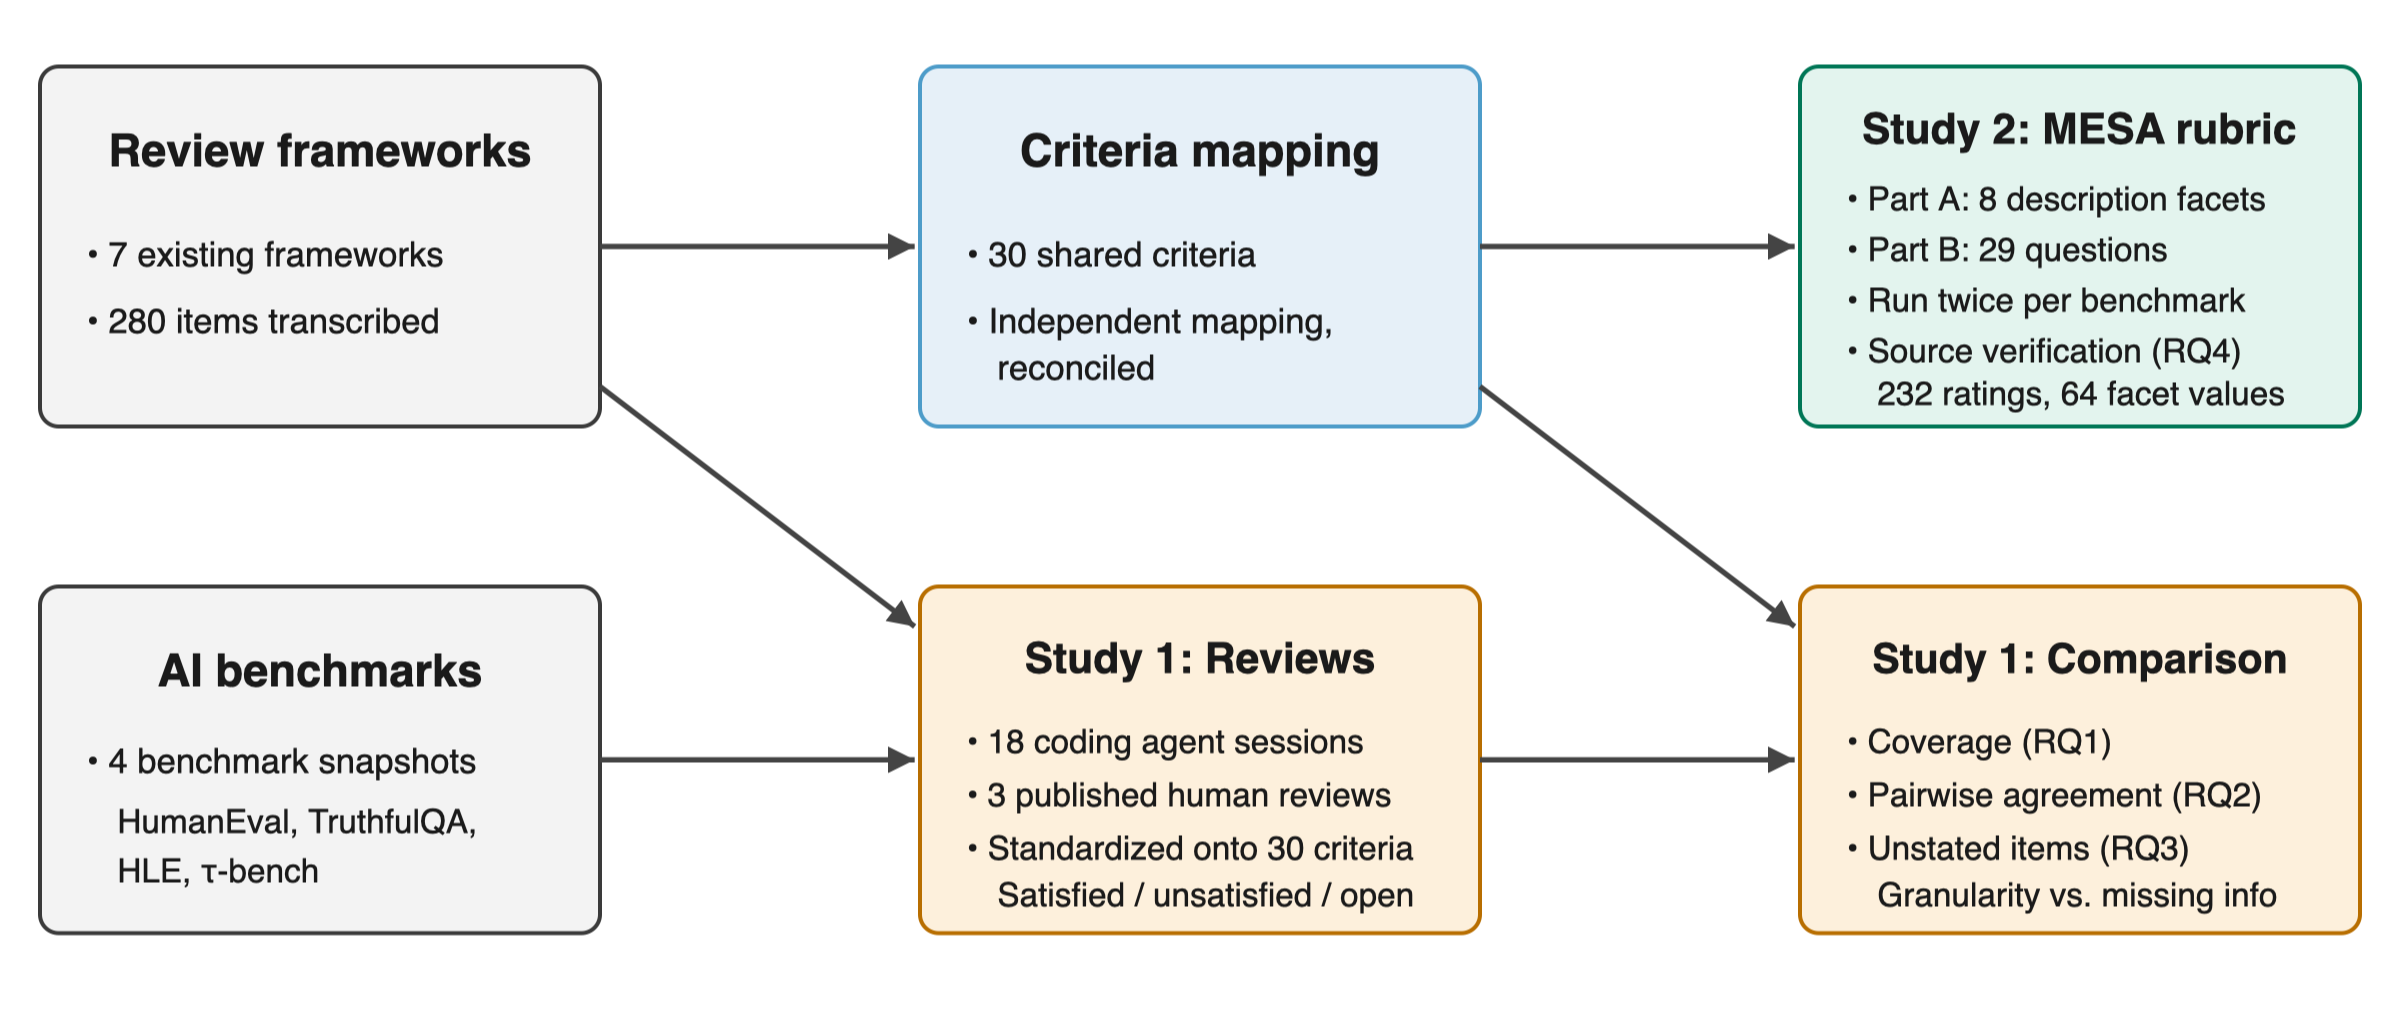
\includegraphics[width=0.82\textwidth]{figures/v4_chase_design.png}
\caption{Study design. Inputs (grey) are mapped to the MESA standard (blue). Study~1 (orange) applies six frameworks to four benchmarks and compares coverage, agreement and treatment of unstated information (RQ1--RQ3). Study~2 (green) applies the derived rubric twice per benchmark and verifies its ratings against sources (RQ4).}
\label{fig:design}
\end{figure*}

\subsection{Benchmarks, frameworks and sessions}
We evaluate four benchmarks plus a two-task fictional fixture (AddTwo) used only for harness pilots before freezing inputs: (1)~\textbf{HumanEval} \cite{human_eval_repository}: 164 Python code generation problems (35-page paper, 12 repo files, 41k--44k tokens), with published reviews in BetterBench and How2Bench, running candidate code through an unrestricted execution call; (2)~\textbf{TruthfulQA} \cite{truthfulqa_repository}: 817 questions testing truthfulness (39-page paper, 25 repo files, 37k--40k tokens), with an earlier 47-item BetterBench review, whose scoring module appends a fallback answer when absent; (3)~\textbf{Humanity's Last Exam (HLE)} \cite{phan_etal_hle_2025}: 2,500 frontier academic questions (29-page paper, 16 repo files, 29k--32k tokens), with gated dataset text included locally under access terms; and (4)~\textbf{$\tau$-bench} \cite{tau_bench_repository}: tool-using agents in simulated airline/retail domains (50-page paper, 113 repo files, 36k--39k tokens), with an earlier ABC review on 31 of 44 items.

In Study~1, the four general frameworks (BetterBench, ECBD, Scorecard, OECD facets) run on all four benchmarks (16 sessions), How2Bench runs on HumanEval (1 session) and ABC runs on $\tau$-bench (1 session), totaling 18 sessions. Caliper requires a declared target region and is mapped in RQ1 without session runs. In Study~2, the MESA rubric runs twice per benchmark (8 sessions), giving 26 main sessions. A recorded post-hoc amendment added a second repetition of BetterBench and Scorecard on HumanEval (2 sessions) to estimate same-framework repeat variation in Section~\ref{sec:rq2}.

\subsection{Agent isolation, pre-experiment checks and hypotheses}
All sessions used Claude Sonnet 5.5 through the Claude Code CLI at medium effort \cite{anthropic_claude_code_cli}. Each session ran in an empty directory with skills and built-in tools disabled and only two read-only tools over the frozen snapshot: listing files and reading numbered lines. Prompts supplied the study instructions, verbatim framework items, a fictional benchmark example, and extracted benchmark texts; responses were schema-validated. Ten pre-experiment checks passed in order before freezing all 254 input files. All 35 attempts (7 pilots, 26 main, 2 amendment) succeeded first time and passed validation. The 26 main sessions took 21 minutes in all (3.87M input, 199k output tokens) and made 50 repository tool calls across 19 sessions, 13 of which read at least one file (6/7 HumanEval, 5/6 HLE, 1/6 TruthfulQA, 1/7 $\tau$-bench).

Five hypotheses were registered in the study protocol before the sessions. H3 was drawn from the coverage table and serves as a descriptive check, and H4 follows partly from the rubric's design and serves as a consistency check: \textbf{H1:} Frameworks agree on documentation/licensing (C18, C19) and diverge on validity criteria (C01--C16); \textbf{H2:} Disagreement on validity criteria stems largely from rules for undocumented items (\emph{undocumented}) rather than reading sources differently; \textbf{H3:} Maintenance/contact (C22, BetterBench), result presentation (C26, How2Bench) and instrument classification (C30, OECD) each appear in one framework only; \textbf{H4:} The MESA rubric records undocumented items as \emph{Undocumented} (\emph{open}) where BetterBench and How2Bench record failures (\emph{unsatisfied} with \emph{undocumented}); and \textbf{H5:} Rubric questions tied to low-agreement OECD facets (B01/B16, B04, B13) are least often confirmed by source verification. Offline analysis deterministically checks citations, standardizes and aggregates verdicts, and evaluates agreement.

\subsection{Verifying ratings against sources}
Source verification evaluated each rubric response, its cited passages, question anchors, and the frozen snapshot. Notes recorded whether cited text was located, searches for missing information, and checks of repository files. Verification labels distinguish support levels: \emph{confirmed} (rating supported), \emph{overstated} (evidence supported a lower level), and \emph{not confirmed} (assigned description unsupported). \emph{Absence plausible} records that an absence or applicability judgment was consistent with inspected material. The assistant recorded a label and reason for each of the 296 entries, and the author verified these findings.

\section{Results}
\subsection{RQ1: Coverage of shared criteria}
\label{sec:rq1}
Table~\ref{tab:coverage} maps the 280 items onto the 30 criteria: 180 items map to one criterion, 94 to two, and 6 to three (SC-26 on design rationale and real world prediction, ABC-T.1 on tool versions, ABC-O.f.3 on preventing flaky tests, ABC-R.4 on updating tasks against overfitting, and the OECD Reproducibility and Variation facets), yielding 386 links. Four structural findings emerge:
\begin{enumerate}
\item \textbf{No criterion is covered by all seven frameworks, and breadth ranges from 10 to 22 criteria.} Caliper covers 10 criteria and ECBD covers 14, while even the broadest frameworks—Scorecard (22), BetterBench (21) and How2Bench (20)—omit at least eight criteria asked by peers. Seven criteria appear in six frameworks, 6 in five, 7 in four, 3 in three, 4 in two, and 3 in one framework only, as expected from the coverage table (H3): maintenance/contact in BetterBench (C22, 4 items), result presentation in How2Bench (C26, 6 items) and instrument classification in OECD (C30, 10 items).
\item \textbf{Granularity is skewed across criteria.} Six criteria absorb 164 of 386 links: task and answer checks (C05, 33), anti-gaming checks (C07, 29), regional transfer (C23, 29), repeatability materials (C18, 28), confounds (C13, 23) and task coverage (C04, 22), while submission rules (C15) and licensing (C19) receive 2 and 3.
\item \textbf{Item counts within a single criterion vary sharply across frameworks.} On C07 (scoring implementation checks), BetterBench, ECBD and How2Bench ask 1 item each, Scorecard asks 8, and ABC asks 18. On C05 (task/answer checks), BetterBench asks 1 item (BB-42) against 10 in Scorecard and 12 in ABC. Under any-unsatisfied aggregation, a framework asking 12--18 narrow items sets a steeper bar than one asking a single question.
\item \textbf{Independent mapping reconciliation resolved 100 item differences.} Author and assistant model mappings matched on 180 of 280 items and differed on 100, mainly on secondary criteria (56 kept the draft, 28 the author's reading, 4 the union, 12 a reconciled reading).
\end{enumerate}

\begin{table*}[t]
\caption{Items per shared criterion and framework.}
\label{tab:coverage}
\centering
\scriptsize
\setlength{\tabcolsep}{3.5pt}
\begin{tabular}{@{}llrrrrrrrr@{}}
\toprule
\textbf{Id} & \textbf{Criterion (rubric question)} & \textbf{BB} & \textbf{ECBD} & \textbf{SC} & \textbf{H2B} & \textbf{ABC} & \textbf{CAL} & \textbf{OECD} & \textbf{Frameworks} \\
\midrule
C01 & The ability under test is stated and made concrete (B01) & 2 & 2 & 3 & 2 & 1 &  & 1 & 6 \\
C02 & The intended use, users and real-world relevance are stated (B02) & 2 & 3 & 1 & 1 & 1 &  & 2 & 6 \\
C03 & Task selection is justified for the claimed ability (B03) & 4 & 3 & 5 & 2 & 1 &  &  & 5 \\
\midrule
C04 & The task set covers the ability and is representative (B04) & 2 & 5 & 4 & 5 &  & 5 & 1 & 6 \\
C05 & Tasks and reference answers were checked (B05) & 1 &  & 10 & 7 & 12 & 3 &  & 5 \\
\midrule
C06 & The scoring rule is described (B06) & 3 & 2 & 4 & 4 & 3 &  & 1 & 6 \\
C07 & The scoring implementation was checked and cannot be gamed (B07) & 1 & 1 & 8 & 1 & 18 &  &  & 5 \\
C08 & Aggregation and subscores are justified (B08) &  & 3 & 3 & 1 &  & 1 & 1 & 5 \\
C09 & Comparison points are justified (B09) & 3 &  & 3 &  & 2 &  & 1 & 4 \\
\midrule
C10 & Variation on repeated testing is reported (B10) &  &  & 2 & 3 & 1 &  & 2 & 4 \\
C11 & Prompting and setup are described and their effect tested (B11) & 2 & 3 & 3 & 6 &  &  &  & 4 \\
C12 & Uncertainty and statistical support are reported (B12) & 1 & 2 & 3 & 1 & 2 &  &  & 5 \\
C13 & Shortcuts, confounds and chance were investigated (B13) &  & 1 & 12 & 1 & 6 & 2 & 1 & 6 \\
\midrule
C14 & Exposure of test material in training data was assessed (B14) & 2 &  & 1 & 1 & 2 &  &  & 4 \\
C15 & Rules for training on the test and for repeated submission are stated (B15) & 1 &  &  &  & 1 &  &  & 2 \\
C16 & Claims about performance beyond the test are supported (B16) & 1 & 1 & 6 & 1 &  & 1 & 2 & 6 \\
C17 & Fairness across systems and conditions is addressed (B17) &  & 1 & 1 &  &  & 1 & 2 & 4 \\
\midrule
C18 & Materials and instructions for repeating the evaluation are provided (B18) & 10 &  & 3 & 11 & 3 &  & 1 & 5 \\
C19 & Terms of access and license are stated (B19) & 1 &  &  & 2 &  &  &  & 2 \\
C20 & Versions and changes are recorded (B20) & 3 &  & 1 &  & 3 &  & 2 & 4 \\
C21 & Limitations and flaws are stated and claims stay within the evidence (B21) & 4 &  & 6 &  & 4 &  &  & 3 \\
C22 & Maintenance and a contact exist (B22) & 4 &  &  &  &  &  &  & 1 \\
\midrule
C23 & Transfer to another cultural or deployment context is assessed (B23) &  &  &  &  &  & 28 & 1 & 2 \\
C24 & Harmful or sensitive content is handled (B24) & 1 &  &  & 3 &  & 1 &  & 3 \\
C25 & The systems evaluated and the difficulty of the benchmark are examined (B25) &  &  &  & 6 &  &  & 1 & 2 \\
C26 & Results are presented and explained (B26) &  &  &  & 6 &  &  &  & 1 \\
C27 & Data provenance and collection are documented (B27) & 7 & 1 & 4 & 5 &  & 1 & 2 & 6 \\
C28 & The evaluation environment is controlled and isolated from answers (B28) &  &  & 3 &  & 7 &  & 1 & 3 \\
C29 & Domain experts or users took part in design or review (B29) & 1 & 1 & 2 &  &  & 2 &  & 4 \\
\midrule
C30 & What kind of instrument the benchmark is, recorded as a description &  &  &  &  &  &  & 10 & 1 \\
\midrule
\multicolumn{2}{@{}l}{Total items in framework / Total item-to-criterion links} & 47 / 56 & 20 / 29 & 68 / 88 & 55 / 69 & 44 / 67 & 28 / 45 & 18 / 32 & 280 / 386 \\
\multicolumn{2}{@{}l}{Criteria covered (out of 30)} & 21 & 14 & 22 & 20 & 16 & 10 & 17 & --- \\
\bottomrule
\end{tabular}
\par\vspace{2pt}\raggedright\footnotesize The question in parentheses is the MESA rubric's evaluation question for the criterion. C30 has no evaluation question: the rubric records it through its description facets. An empty cell means no item.
\end{table*}

\subsection{RQ2: Agreement across frameworks}
\label{sec:rq2}
The 18 Study 1 sessions produced 711 item answers (52 descriptive OECD facet answers are not standardized). Table~\ref{tab:grid-humaneval} shows the standardized criterion verdicts on HumanEval. Three framework patterns stand out across all four benchmarks: the Scorecard is unsatisfied on most covered criteria, mostly by its rule for undocumented items (123 of its 272 answers rest on absent information); ECBD is never unsatisfied, since it records an undocumented item as open; and BetterBench sits between them, satisfied (partial) on many validity criteria and unsatisfied under the framework's rule on C14, C18, C20 and C22 on every benchmark.

\begin{table}[t]
\caption{Verdicts per criterion on HumanEval.}
\label{tab:grid-humaneval}
\centering
\footnotesize\begin{tabular}{@{}lcccccc@{}}\toprule
\textbf{Criterion} & \textbf{BB} & \textbf{ECBD} & \textbf{SC} & \textbf{H2B} & \textbf{OECD} & \textbf{Rubric} \\
\midrule
C01 / C02 & (+) / -r & (+) / (+) & + / ? & + / + & d / d & (+) / (+) \\
C03 / C04 & (+) / -r & (+) / (+) & -r / -r & + / -r & -- / - & (+) / (+) \\
C05 / C06 & ? / -r & -- / + & -r / -r & -r / -r & -- / d & ? / (+) \\
C07 / C08 & (+) / -- & + / (+) & -r / -r & -r / -r & -- / d & (+) / (+) \\
C09 / C10 & -r / -- & -- / -- & -r / -r & -- / -r & d / - & (+) / (+) \\
\midrule
C11 / C12 & (+) / (+) & (+) / (+) & -r / -r & -r / ? & -- / -- & + / ? \\
C13 / C14 & -- / -r & + / -- & -r / -r & -r / + & - / -- & (+) / (+) \\
C15 / C16 & -r / (+) & -- / + & -- / -r & -- / + & -- / d & ? / (+) \\
C17 / C18 & -- / -r & ? / -- & ? / -r & -- / -r & - / - & (+) / (+) \\
C19 / C20 & + / -r & -- / -- & -- / ? & + / -- & -- / - & (+) / ? \\
\midrule
C21 / C22 & -r / -r & -- / -- & -r / -- & -- / -- & -- / -- & (+) / (+) \\
C23 / C24 & -- / -r & -- / -- & -- / -- & -- / -r & - / -- & ? / (+) \\
C25 / C26 & -- / -- & -- / -- & -- / -- & -r / -r & d / -- & (+) / + \\
C27 / C28 & -r / -- & + / -- & ? / -r & -r / -- & d / d & (+) / (+) \\
C29 / C30 & -r / -- & ? / -- & -r / -- & -- / -- & -- / d & ? / -- \\
\bottomrule\end{tabular}
\par\vspace{2pt}\raggedright\footnotesize Two criteria per row, left and right of the slash. +: satisfied; (+): satisfied (partial); -: unsatisfied; ?: open; d: descriptive only; r: unsatisfied by the framework's rule for undocumented items; --: no item. The last column is the MESA rubric, repetition 1, for reference.
\end{table}

\begin{table}[t]
\caption{Agreement between framework pairs per benchmark.}
\label{tab:pairwise}
\centering
\footnotesize\begin{tabular}{@{}lrrrr@{}}\toprule
\textbf{Pair} & \textbf{HumanEval} & \textbf{TruthfulQA} & \textbf{HLE} & \textbf{$\tau$-bench} \\
\midrule
BB and ECBD & 6/11 (4) & 9/11 (7) & 7/11 (6) & 7/11 (3) \\
BB and SC & 8/17 (7) & 10/17 (7) & 7/17 (6) & 10/17 (8) \\
BB and OECD & 3/3 (3) & 0/3 (0) & 2/3 (2) & 2/3 (2) \\
BB and H2B & 9/15 (6) &  &  &  \\
\midrule
ECBD and SC & 2/14 (1) & 6/14 (3) & 4/14 (3) & 3/14 (2) \\
ECBD and OECD & 0/3 (0) & 0/3 (0) & 0/3 (0) & 0/3 (0) \\
ECBD and H2B & 4/12 (1) &  &  &  \\
\midrule
OECD and SC & 4/6 (4) & 4/6 (4) & 5/6 (5) & 4/6 (4) \\
\midrule
H2B and SC & 10/16 (10) &  &  &  \\
H2B and OECD & 4/4 (4) &  &  &  \\
\midrule
ABC and BB &  &  &  & 10/13 (7) \\
ABC and ECBD &  &  &  & 3/7 (1) \\
ABC and SC &  &  &  & 13/15 (12) \\
ABC and OECD &  &  &  & 3/4 (3) \\
\midrule
All pairs & 50/101 (40) & 29/54 (21) & 25/54 (22) & 55/93 (42) \\
\bottomrule\end{tabular}
\par\vspace{2pt}\raggedright\footnotesize Criteria with the same verdict over criteria both frameworks cover, repetition 1; in parentheses, matches that also agree on the \emph{partial} qualifier.
\end{table}

Across all 32 framework pairs and 302 shared criterion comparisons (Table~\ref{tab:pairwise}), 159 (53\%) reach the same verdict and 125 (41\%) also match on the \emph{partial} qualifier. This is agreement between MESA translations within shared review topics. It depends on the mapping and aggregation rule, and a mismatch can reflect different requirements rather than conflicting readings of the evidence. The majority-rule count tests the effect of aggregation; it does not establish that the mapped requirements are equivalent. Audit checklists that share a penalizing rule for undocumented items agree more (ABC and Scorecard: 13/15 on $\tau$-bench; How2Bench and Scorecard: 10/16 on HumanEval) than pairs whose rules diverge (ECBD and Scorecard: 2--6 of 14; ECBD and OECD evaluative facets: 0/3 on all benchmarks). Some pairs with OECD evaluative facets agree fully (BetterBench 3/3 and How2Bench 4/4 on HumanEval), but on few comparisons. Excluding the 14 pairs involving OECD evaluative facets (31/56 agreements), the remaining 18 pairs agree on 128 of 246 comparisons. Replacing any-unsatisfied aggregation with a majority rule (ties unsatisfied) yields 148 of 302 agreements, so the overall agreement level changes little under this alternative rule.

In the HumanEval amendment, repeating BetterBench matched its first run on 19 of 21 criteria (40/47 items) and repeating the Scorecard on 20 of 22 (56/68 items), well above the 8 of 17 agreement between the two frameworks on that benchmark; all four changes involved the \emph{undocumented} qualifier. Hypothesis H1 holds in direction: pairs agree on 17 of 19 comparisons on documentation and licensing (C18, C19), versus 117 of 221 on validity criteria (C01--C16) and 25 of 62 on remaining criteria. Most of the C18 and C19 agreements are shared unsatisfied verdicts rather than shared positive judgments, and the remaining criteria agree less than the validity criteria.

\begin{table}[t]
\caption{Disagreement causes and source verification findings.}
\label{tab:disagreements-sourceverification}
\centering\footnotesize
\begin{tabularx}{\columnwidth}{@{}Xrr@{}}
\toprule
\multicolumn{3}{@{}l}{\textbf{Panel A: Disagreement Causes (Study 1, $N=143$)}} \\
\midrule
\textbf{Cause category} & \textbf{Total} & \textbf{Undocumented ($-r$)} \\
\midrule
Item granularity & 50 & 37 \\
Rule for undocumented items & 42 & 42 \\
Reading of criterion & 42 & 18 \\
Evidence threshold & 8 & 0 \\
Sources read & 1 & 0 \\
\midrule
\multicolumn{3}{@{}l}{\textbf{Panel B: Source Verification Findings (Study 2, $N=296$)}} \\
\midrule
\textbf{Verification outcome} & \textbf{Eval (232)} & \textbf{Facet (64)} \\
\midrule
Confirmed & 190 & 45 \\
Overstated & 21 & 18 \\
Absence plausible & 21 & 0 \\
Not confirmed & 0 & 1 \\
\bottomrule
\end{tabularx}
\par\vspace{2pt}\raggedright\footnotesize Panel~A: causes of the 143 Study~1 verdict differences. Panel~B: source verification findings across 296 Study~2 rubric ratings and description facets.
\end{table}

\textbf{Explanations of disagreement.} Of the 143 disagreements, 97 involve an unsatisfied verdict qualified as \emph{undocumented} on at least one side (85 vs.\ satisfied, 12 vs.\ open), while 46 do not (29 satisfied vs.\ unmarked unsatisfied, 11 satisfied vs.\ open, 6 unmarked unsatisfied vs.\ open). As shown in Table~\ref{tab:disagreements-sourceverification} (Panel~A), verified coding against five pre-specified categories attributed 92 differences to \emph{item granularity} (50, narrow items deciding multi-item criteria) or \emph{rules for undocumented items} (42, identical absences scored differently). Differing \emph{readings of the criterion} accounted for 42 differences, evidence \emph{threshold} for 8, and \emph{sources read} for 1 (inspecting dependencies on $\tau$-bench). Among the 97 disagreements involving the undocumented qualifier ($-r$), 42 were assigned to rules for undocumented items, 37 to granularity and 18 to reading. H2 thus receives partial support: while unstated information drives many splits, reading and threshold differences (50 cases) confirm that interpretation divergence remains substantial.

\textbf{A worked example.} Criterion C12 (statistical support) on HumanEval illustrates these mechanics. BetterBench asks BB-22 (uncertainty quantification); the agent scored it 10 because the paper proves an unbiased pass@k estimator with 200 samples without confidence intervals, yielding satisfied (partial). The Scorecard asks three items: SC-13 (estimator) is satisfied on the same passage, while SC-14 (power) and SC-15 (confidence intervals) are unsatisfied, yielding unsatisfied with the \emph{undocumented} qualifier under any-unsatisfied aggregation. ECBD credits the unbiased proof (Q20) while noting absent validity evidence (Q14), yielding satisfied (partial). How2Bench (H2B-09, sampling) was judged inapplicable (open). All four cite Section~2.1 and Appendix~A without disputing facts; disagreements reflect required evidence and item allocation.

\textbf{Comparison with published human reviews and repository inspection.} The framework teams' own published reviews are the study's human reference point. On the 21 BetterBench criteria, the agent matched the BetterBench authors' published reviews on 15 criteria for HumanEval (11 strict) and 17 for TruthfulQA (13 strict); all four TruthfulQA differences were unsatisfied under the framework's rule in the published review and satisfied in the agent review of the 2025 repository. Every unsatisfied BetterBench criterion in both agent and author reviews carried the \emph{undocumented} qualifier. Six of seven HumanEval sessions read the execution module, but only one (rubric repetition 2, B28 \emph{Contradicted}) caught that the repository documentation claims execution is commented out while the call is active; rubric repetition 1 echoed the documentation. On TruthfulQA, only BetterBench read a repository file, and no session opened the scoring module where fallback answers are appended.

\subsection{RQ3: Information a benchmark does not report}
\label{sec:rq3}
Table~\ref{tab:frameworks} shows the structural split across the seven frameworks: five (BetterBench, Scorecard, How2Bench, ABC and Caliper at the dimension level) penalize undocumented items by design, whereas two (ECBD and OECD on Reliability) record undocumented items without a negative score.

\begin{table}[t]
\caption{Standardized verdicts of the published reviews.}
\label{tab:earlier-reviews}
\centering
\footnotesize
\setlength{\tabcolsep}{2.5pt}
\begin{tabularx}{\columnwidth}{@{}l>{\raggedright\arraybackslash}Xrrrrr@{}}
\toprule
\textbf{Benchmark} & \textbf{Review} & \textbf{+} & \textbf{(+)} & \textbf{--r} & \textbf{--} & \textbf{?} \\
\midrule
HumanEval & BB, 45 items & 26 & 3 & 14 & 0 & 2 \\
 & \emph{21 criteria} & \emph{9} & \emph{0} & \emph{11} & \emph{0} & \emph{1} \\
\midrule
TruthfulQA & BB, 45 items & 22 & 8 & 15 & 0 & 0 \\
 & \emph{21 criteria} & \emph{7} & \emph{3} & \emph{11} & \emph{0} & \emph{0} \\
\midrule
$\tau$-bench & ABC, 31 items & 17 & 0 & 9 & 2 & 3 \\
 & \emph{15 criteria} & \emph{5} & \emph{2} & \emph{6} & \emph{2} & \emph{0} \\
\bottomrule
\end{tabularx}
\par\vspace{2pt}\raggedright\footnotesize Unanswerable items BB-45 and BB-46 excluded. The first row per benchmark counts items, the italic row aggregates them to criteria. +: satisfied; (+): satisfied (partial); --r: unsatisfied by the rule for undocumented items; --: unsatisfied for a defect; ?: open / not applicable.
\end{table}

Standardizing the three published item-level reviews (Table~\ref{tab:earlier-reviews}) confirms this pattern: all 11 unsatisfied BetterBench criteria on HumanEval and TruthfulQA (22/22) carry the \emph{undocumented} qualifier with zero contradicted findings. On $\tau$-bench, 9 of 11 zeros in the ABC review reflect undocumented items, and only 2 record contradicted evidence (empty ground truth allowing guessing).

In Study~1 agent sessions, 9 benchmark-criterion cells (12 framework pairs) show direct conflict between an \emph{unsatisfied} (\emph{undocumented}) verdict and an \emph{open} verdict on the identical absence. Across 711 Study~1 answers, BetterBench, Scorecard, How2Bench and ABC recorded 199 answers with absent information (41, 123, 23, 12) and only 13 with contradicted evidence (2, 9, 0, 2). Separately, 210 answers (30\%) carry the \emph{undocumented} qualifier (52/188 BB, 123/272 SC, 23/55 H2B, 12/44 ABC). Negative scores for missing reports outnumber documented defects by more than ten to one. Because agents read few repository files and missed known defects (Section~\ref{sec:rq2}), the count of contradicted evidence is a lower bound.

\subsection{RQ4: The MESA rubric}
\label{sec:rq4}
The eight Study~2 rubric sessions produced 64 description facet values (Part~A) and 232 evaluation question ratings (Part~B): 123 \emph{Documented}, 52 \emph{Verified}, 20 \emph{Undocumented}, 18 \emph{Not applicable}, 14 \emph{Claimed}, and 5 \emph{Contradicted} (HumanEval active execution vs.\ documentation on B28; 164 tasks vs.\ 158 in appendix on B20; HLE filtering on B17; and $\tau$-bench claiming error bars absent in results on B12).

\textbf{Citations and source verification.} The 232 evaluation ratings carried 271 citations (1.2 per rating; 260 named snapshot files, 232 quoted source text, 236 carried line/page locators). As summarized in Table~\ref{tab:disagreements-sourceverification} (Panel~B), source verification confirmed 190 of 232 evaluation ratings, found 21 overstated, 21 absence-plausible (all 18 \emph{Not applicable}), and 0 unconfirmed. Among the 64 description facets, 45 were confirmed, 18 overstated, and 1 unconfirmed, with errors concentrated on \emph{Objectivity} (7/8 rated \emph{customised} for fixed tests) and \emph{Variation} (5/8 rated \emph{altered} for later releases). \emph{Objectivity} was placed in Part~A because OECD raters agreed on it consistently, so its error rate here is a limitation of the Part~A design. These facets gate questions only when applicability changes: \emph{Objectivity} gates nothing, and B20 applies whenever releases exist. Overstated \emph{Reference} on $\tau$-bench (repetition 2) shifted B09's evaluated scope to relative comparison; the saved rating was \emph{Undocumented}. Contrary to H5, low-agreement OECD facets were confirmed in 8/8 cases on B01, B04, B13 and 6/8 on B16, whereas B02, B07, B12, and B25 had the most overstated ratings (5/8 confirmed each).

\textbf{Repeatability and undocumented items.} Across the two repetitions, 93 of 116 repeated evaluation ratings (80\%) received identical levels (21/29 HumanEval, 24/29 TruthfulQA, 22/29 HLE, 26/29 $\tau$-bench), with 19 of 23 differences between adjacent levels (\emph{Verified} vs.\ \emph{Documented} 12; \emph{Documented} vs.\ \emph{Claimed} 7). Description facets agreed on 29 of 32 repeated values. Consistent with H4, which follows partly from the rubric's design, of the 29 rubric ratings whose evidence was undocumented, 20 were recorded as \emph{Undocumented}, 9 as \emph{Claimed} (crediting stated principles without inspectable artifacts), and none as \emph{Contradicted}, whereas all 199 such answers in BetterBench, How2Bench, Scorecard, and ABC were scored unsatisfied under framework rules. Under Table~\ref{tab:standardization}, the 9 \emph{Claimed} ratings count as satisfied (partial).

\section{Discussion}
\textbf{Why benchmark reviews disagree.} Differences in framework requirements and scoring rules drive disparate verdicts. Five of the seven mapped frameworks penalize undocumented items by design. In Study~1, 210 of 711 answers and 109 of 149 unsatisfied criterion verdicts carried the undocumented qualifier. Across BetterBench, Scorecard, How2Bench and ABC, 199 answers recorded absent information while only 13 recorded contradicted evidence; this ratio likely undercounts defects, since agents read few repository files (Section~\ref{sec:rq2}). Because frameworks allocate 1 to 18 items per criterion, a single unsatisfied narrow item can trigger an unsatisfied criterion verdict under any-unsatisfied aggregation. Verified coding assigned 92 of 143 differences to item granularity (50) or unstated-information rules (42). In contrast, same-framework repeats on HumanEval matched on 19/21 (BetterBench) and 20/22 criteria (Scorecard), suggesting that inter-framework divergence reflects instrument design rather than stochastic agent variation, although this rests on one repeat of two frameworks on one benchmark.

\textbf{A review scenario.} Suppose a team audits HumanEval to select a code generation component. One engineer applies the Scorecard, while another uses ECBD. Their verdicts on uncertainty conflict: the Scorecard marks the criterion unsatisfied for lack of confidence intervals and power justification, whereas ECBD credits proof of an unbiased estimator. The proof confirms estimator properties but does not establish whether observed differences between candidate models are statistically discernible. MESA reconciles both assessments into a single record of requirements and cited evidence, enabling engineers to identify what missing information their decision requires. The shared record also changes the team's discussion: instead of debating which framework is right, members can agree on which missing evidence matters for their decision, and keep \emph{not reported} separate from \emph{shown to be wrong} when they record the outcome.

\textbf{Implications for review teams.} For teams that combine reviewers or frameworks, the 30 criteria and the qualifiers give a common format for pooling verdicts and tracing disagreements to their source. For benchmark users, frameworks that penalize omissions conflate missing documentation with empirical defects. MESA separates unstated practices from verified contradictions while exposing the limits of static inspection: only one session flagged HumanEval's active execution call and none examined TruthfulQA's scoring module. For creators, the 29 evaluation questions clarify evidence thresholds needed to advance claims to documented artifacts (\emph{Documented}, 123 ratings) and verified checks (\emph{Verified}, 52 ratings). For framework designers, mapping onto 30 criteria enables cross-framework comparison without obscuring underlying requirements.

\section{Threats to Validity}
\textbf{Construct validity.} The 30 criteria and standardization rules represent interpretive artifacts from author reconciliation of an assistant draft; all mappings and notes are published. Comparisons are restricted to shared criteria, and majority-rule aggregation sensitivity is reported (148 vs.\ 159 of 302). Table~\ref{tab:standardization} maps BetterBench score 5 (mentioned without evidence) to unsatisfied (\emph{undocumented}) but the rubric's \emph{Claimed} to satisfied (\emph{partial}); the rules are kept as registered, and this asymmetry widens the contrast between the rubric and the frameworks.

\textbf{Internal validity.} The MESA rubric was derived before study sessions and excluded from Study~1 agreement counts. Same-framework variation was evaluated on HumanEval only. H3 was drawn from the coverage table and H4 follows partly from the rubric's design, so neither is an independent test. Standardization relied on agent-recorded evidence fields verified by the author rather than independent external raters.

\textbf{External validity.} Findings are bounded by four benchmarks, one agent model configuration, text extraction lacking figure layout, and read-only repository inspection. Because one model applied every framework, Study~1 measures framework design together with one reviewer, not human review practice. Agents read repository files in 13 of 26 sessions, so contradicted evidence is a lower bound. Published BetterBench reviews predate TruthfulQA's 2025 update, and ABC authors scored 31 of 44 items on $\tau$-bench.

\textbf{Conclusion validity and researcher bias.} Mapping drafts, analysis scripts, disagreement coding, and source verification were prepared by an assistant model from the same family as the reviewer agent, followed by author verification. These checks do not constitute independent human validation.

\section{Conclusion and Future Work}
The seven frameworks examined lacked common ground: they asked overlapping questions on divergent scales with conflicting rules for unstated information. MESA bridges this divide by providing a shared vocabulary of 30 criteria, standardized verdicts with qualifiers that decouple missing reporting from confirmed defects, and verifiable answer records. Applying six frameworks to four benchmarks revealed that, in agent answers, penalties for unstated information outnumber documented defects by over ten to one, a ratio limited by how little code the agents inspected, and that 92 of 143 cross-framework disagreements stem from scoring conventions or item granularity. The derived MESA rubric demonstrated 80\% repeatability across runs, and source verification confirmed 190 of its 232 ratings, with 21 overstated. Future work will evaluate the rubric with human software engineering teams and refine anchors for mixed evidence.

\section*{Data Availability}
Study materials, snapshots, and analysis records are available anonymously: \url{https://example.org/anonymous-artifact}.

\section*{Disclosure of Generative Model Use}
Claude Fable 5.1 assisted in item transcription, mapping and rubric drafting, analysis scripting, and source verification. The author verified all coding, analyses, and findings, and edited the manuscript. Claude Sonnet 5.5 served as the reviewer agent across all study sessions.
\bibliographystyle{IEEEtran}
\bibliography{references}
% Future extension alongside human participation:
% Revisit the 143 verdict differences and classify each as concerning
% equivalent requirements, different requirements, or an unclear case.
% Record the item wording, evidence and reasons for each classification.
% Allow more than one explanation where categories overlap.
% Preserve the original coding and store this analysis separately.
% Document who performs and checks the analysis, and report counts
% without treating the comparisons as independent observations.
% Plan the human study before recruitment, including its population,
% consent, recruitment, exclusions and analysis decisions.
% Before a future rubric version is used, clarify which upper anchors
% require a check and which require more complete documentation, and
% specify how to record a check that also reports a defect.
% Freeze those changes before further sessions; do not restandardize this study.
% Future source verification should define a consistent search scope and a rule
% for supporting and conflicting evidence before checking new responses.
% Further future studies (not run; no new data in this version):
% Report chance-corrected agreement (Cohen's kappa, weighted kappa or
% Krippendorff's alpha) for the author and draft mappings, the rubric
% repeats and the BetterBench and Scorecard repeats, with intervals
% clustered by benchmark.
% Run a sensitivity standardization that maps BetterBench score 5 like
% the rubric's Claimed level, reported beside the frozen results.
% Compare only items judged to ask the same thing, to separate item
% granularity from the any-unsatisfied aggregation rule.
% Tabulate known defects (HumanEval active execution call, 164 vs. 158
% tasks, TruthfulQA fallback answer, tau-bench empty ground truth) and
% which sessions detected each one and opened the relevant file.
% Have a second human coder code the 143 disagreement causes and a
% stratified sample of the source checks, and report agreement.
% Run a small human application study (BetterBench, Scorecard and the
% rubric on HumanEval), planned before recruitment.
% This extension is future work, not required to complete the CHASE study.
\end{document}
